\newpage


% \section{List Scheduling}


\section{Instruction Scheduling}


\subsection{List Scheduling}

List scheduling is a high-level scheduling technique that operates on a basic block of code. The goal of list scheduling is to assign a relative order to the instructions in the basic block so that the dependencies between them are respected and the execution time is minimized. List scheduling considers only the instructions within the basic block and does not take into account the other blocks of code that the program may contain.

\subsection{Global Instruction Scheduling}

Global instruction scheduling, on the other hand, is a more advanced low-level scheduling technique that considers the entire program rather than just a basic block of code. It attempts to schedule instructions from all basic blocks in the program to minimize the total execution time. Global instruction scheduling can reorder instructions across basic blocks and make use of available resources, such as pipelining and parallelism, to improve performance.



\begin{algorithm}
	\caption{Iterative Algorithms}\label{alg:Global Instruction Scheduling}
	\begin{algorithmic}
		\State {Step 0: Compute data dependencies between instructions.}
		\State {Step 1: Figure out code motions that are always better.}
		\State {Step 2: Figure out the probability of each code path to identify hot code paths.}
		\State {Step 3: Speculate. }
	\end{algorithmic}
\end{algorithm}



\begin{problem} Global Instruction Scheduling

	\item Assume you have a machine with a statically scheduled processor that can only issue one operation every
	clock. All operations have a latency of one clock cycle, with the exception of its memory load
	operation, which has a latency of three clock cycles. Consider the following locally scheduled
	program:
	\begin{center}
		\begin{tikzpicture}
			\node[bb, text width=9em, label=left:L0] (l0)  {$d$ = $*a$;\\\texttt{nop};\\\texttt{nop};\\\texttt{if} ($d \ge 0$) \texttt{goto} L1;};
			\node[bb, text width=9em, below left=2em and 3em of l0, label=left:L1] (l1) {\texttt{if} ($d == 0$) \texttt{goto} L3;};
			\node[bb, text width=9em, below right=2em and 3em of l0, label=right:L2] (l2) {$f$ = $*d$; \\\texttt{nop}; \\ \texttt{nop};\\ $k$ = $f+8$;};
			\node[bb, text width=9em, below right=1em and 1em of l1, label=left:L3] (l3) {$k$ = $*d$;\\ \texttt{nop};\\ \texttt{nop};\\ $c$ = $k + k$;};
			\node[bb, text width=9em, below=15em of l0, label=right:L4] (l4) {$w$ = $a + c$; \\ $t$ = $k + w$;};
			\node[bb, below=2em of l4] (exit)  {\exit};
	
			\node[below=8em of l1] {$1 - p$};
			\draw[->] (l0) -- (l1) node [midway, above=10pt] {$p$};
			\draw[->] (l0) -- (l2) node [midway, above=7pt] {$1 - p$};
			\draw[->] (l1) -- (l3) node [midway, below=10pt] {$p$};
			\draw[->] (l2) -- (l4);
			\draw[->] (l3) -- (l4);
			\draw[->] (l1.south) to [out=-90,in=180] (l4.west);
			\draw[->] (l4) -- (exit);
		\end{tikzpicture}
	\end{center}
	All variables in the program are defined before the entry (L0) of the program.
	Assume that only variable $t$ is live at the exit of the program. Each branch in the flow graph is
	labeled with the probability that it is taken dynamically. To answer the following, you may
	apply any of the code motions discussed in class, but no other optimizations.
	
	\begin{enumerate}
		\item Is this the best globally scheduled code that can be generated given that $p = 0.9$? If
		not, provide the improved code along with its expected execution time. \textbf{Note: for an \texttt{if} branch instruction, assume that if the branch corresponding to ``\texttt{goto} L'' is taken, it costs two cycles; otherwise it costs only one.}
	{\color{red}
	
		In the original program, the number of clock cycles and the probability for each path
		are shown as follows:
		\item L0 $\rightarrow$ L1 $\rightarrow$ L4, p = 0.09, num\_cycles = 8
		\item L0 $\rightarrow$ L1 $\rightarrow$ L3 $\rightarrow$ L4, p = 0.81, num\_cycles = 13
		\item L0 $\rightarrow$ L2 $\rightarrow$ L4, p = 0.1, num\_cycles = 10

		The expected execution time is 8 * 0.09 + 13 * 0.81 + 10 * 0.1 = 12.25 cycles.
		We can get a better schedule by pushing the instructions in L4 upwards to fill in the
		idle points when the program is waiting for the result of a memory load.
		
		\begin{center}
			\begin{tikzpicture}
				\node[bb, text width=9em, label=left:L0] (l0)  {$d$ = $*a$;\\ $w$ = $a + c$; \\ $t$ = $k + w$; \\\texttt{if} ($d \ge 0$) \texttt{goto} L1;};
				\node[bb, text width=9em, below left=2em and 3em of l0, label=left:L1] (l1) {\texttt{if} ($d == 0$) \texttt{goto} L3;};
				\node[bb, text width=9em, below right=2em and 3em of l0, label=right:L2] (l2) {$f$ = $*d$; \\\texttt{nop}; \\ \texttt{nop};\\ $k$ = $f+8$;\\ $t$ = $k + w$;};
				\node[bb, text width=9em, below right=1em and 1em of l1, label=left:L3] (l3) {$k$ = $*d$;\\ \texttt{nop};\\ \texttt{nop};\\ $c$ = $k + k$;\\$w$ = $a + c$; \\ $t$ = $k + w$;};
				\node[bb, text width=9em, below=15em of l0, label=right:L4] (l4) {};
				\node[bb, below=2em of l4] (exit)  {\exit};
		
				\node[below=8em of l1] {$1 - p$};
				\draw[->] (l0) -- (l1) node [midway, above=10pt] {$p$};
				\draw[->] (l0) -- (l2) node [midway, above=7pt] {$1 - p$};
				\draw[->] (l1) -- (l3) node [midway, below=10pt] {$p$};
				\draw[->] (l2) -- (l4);
				\draw[->] (l3) -- (l4);
				\draw[->] (l1.south) to [out=-90,in=180] (l4.west);
				\draw[->] (l4) -- (exit);
			\end{tikzpicture}
		\end{center}



		The number of clock cycles and the probability for each path are shown as follows:
\item L0 $\rightarrow$ L1 $\rightarrow$ L4, p = 0.09, num\_cycles = 6
\item L0 $\rightarrow$ L1 $\rightarrow$ L3 $\rightarrow$ L4, p = 0.81, num\_cycles = 13
\item L0 $\rightarrow$ L2 $\rightarrow$ L4, p = 0.1, num\_cycles = 9
The expected execution time is 6 * 0.09 + 13 * 0.81 + 9 * 0.1 = 11.97 cycles.

	}

		\item Repeat part 1, but instead assume that $p = 0.1$.
	
	{\color{red}
	In the original program, the number of clock cycles and the probability for each path
	are shown as follows:
	\item L0 $\rightarrow$ L1 $\rightarrow$ L4, p = 0.09, num\_cycles = 8
	\item L0 $\rightarrow$ L1 $\rightarrow$ L3 $\rightarrow$ L4, p = 0.01, num\_cycles = 13
	\item L0 $\rightarrow$ L2 $\rightarrow$ L4, p = 0.9, num\_cycles = 10
	The expected execution time is 8 * 0.09 + 13 * 0.01 + 10 * 0.9 = 9.85 cycles.
	With the following optimized program:

	\begin{center}
		\begin{tikzpicture}
			\node[bb, text width=9em, label=left:L0] (l0)  {$d$ = $*a$;\\$w$ = $a + c$; \\ $t$ = $k + w$;\\ $k$ = $*d$;\\ \texttt{if} ($d \ge 0$) \texttt{goto} L1;};
			\node[bb, text width=9em, below left=2em and 3em of l0, label=left:L1] (l1) {\texttt{if} ($d == 0$) \texttt{goto} L3;};
			\node[bb, text width=9em, below right=2em and 3em of l0, label=right:L2] (l2) {\texttt{nop}; \\ $k$ = $f+8$; \\ $t$ = $k + w$;};
			\node[bb, text width=9em, below right=1em and 1em of l1, label=left:L3] (l3) {$k$ = $*d$;\\ \texttt{nop};\\ \texttt{nop};\\ $c$ = $k + k$; \\ $w$ = $a + c$; \\ $t$ = $k + w$; };
			\node[bb, text width=9em, below=15em of l0, label=right:L4] (l4) {};
			\node[bb, below=2em of l4] (exit)  {\exit};
	
			\node[below=8em of l1] {$1 - p$};
			\draw[->] (l0) -- (l1) node [midway, above=10pt] {$p$};
			\draw[->] (l0) -- (l2) node [midway, above=7pt] {$1 - p$};
			\draw[->] (l1) -- (l3) node [midway, below=10pt] {$p$};
			\draw[->] (l2) -- (l4);
			\draw[->] (l3) -- (l4);
			\draw[->] (l1.south) to [out=-90,in=180] (l4.west);
			\draw[->] (l4) -- (exit);
		\end{tikzpicture}
	\end{center}

	the number of clock cycles and the probability for each path are shown as follows:
\item L0 $\rightarrow$ L1 $\rightarrow$ L4, p = 0.09, num\_cycles = 7
\item L0 $\rightarrow$ L1 $\rightarrow$ L3 $\rightarrow$ L4, p = 0.01, num\_cycles = 14
\item L0 $\rightarrow$ L2 $\rightarrow$ L4, p = 0.9, num\_cycles = 8
The expected execution time is 7 * 0.09 + 14 * 0.01 + 8 * 0.9 = 7.97 cycles.
	}
	\end{enumerate}
	
	\end{problem}
	


	\begin{problem} Software Pipelining with Register Allocation

		\item Consider the following do-all loop program:
		\begin{verbatim}
		for (i = 0; i < 1000; i++)
			C[i] = (A[i] - b) * A[i];
		\end{verbatim}
		One iteration of the loop can be written in assembly as:
		\begin{verbatim}
		1.  LD   R5, 0(R1++)     // R1 = &A[i]; R5 = *R1; R1++
		2.  SUB  R6, R5, R2      // R2 = b; R6 = R5 - R2
		3.
		4.  MUL  R6, R6, R5      // R6 = R6 * R5
		5.
		6.  ST   R6, 0(R3++)     // R3 = &C[i]; *R3 = R6; R3++
		\end{verbatim}
		Optimize this program using software pipelining for a machine with the following specifications:
		\begin{itemize}[noitemsep]
			\item The processor can issue at most one \texttt{LD} instruction, one \texttt{ST} instruction, and one arithmetic instruction within the same clock cycle.
			\item Each arithmetic operation has a two-cycle latency, but can be pipelined.
			\item The processor supports auto-incrementing addressing and hardware loop operations.
		\end{itemize}
		
		\item Answer the questions below using your optimized program:
		\begin{enumerate}
			\item What is the minimum initiation interval?
			{\color{red} 2}
			\item Write down the pipelined portion of the loop using actual registers. Annotate each instruction with the iteration it's associated with (e.g., $i$, $i+1$, $i+2$, etc.). Resolve any anti-dependencies across loop iterations by unrolling the loop as described in class.
			
\begin{figure}[H]
    \centering
    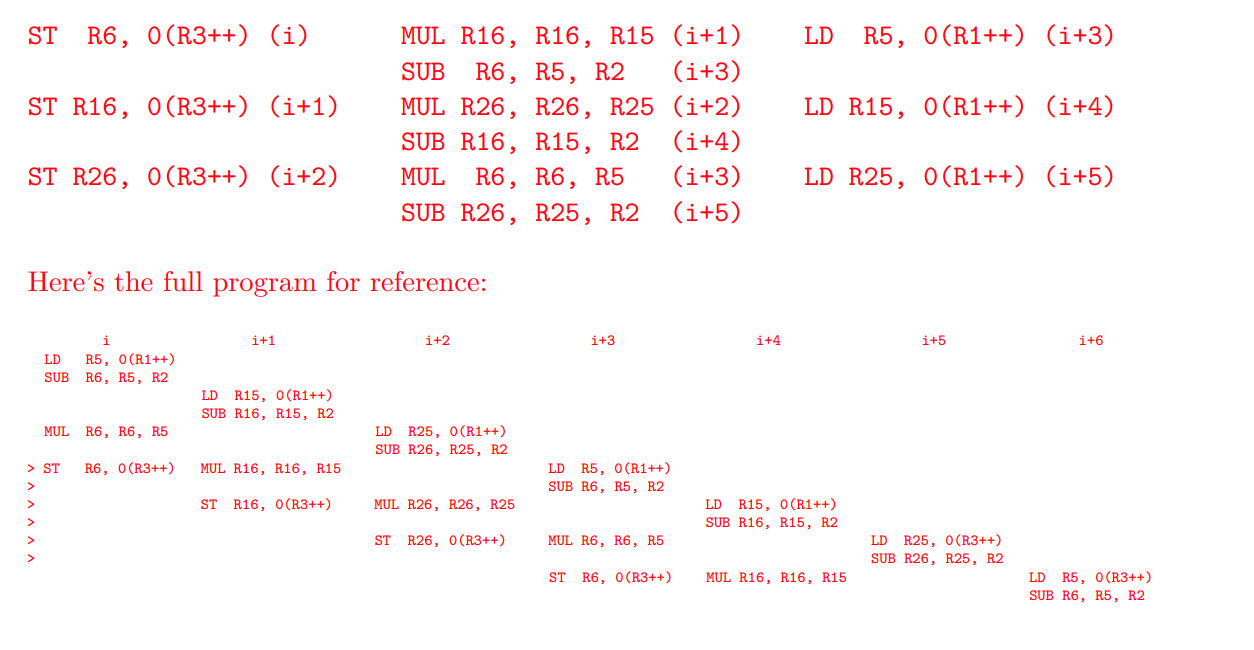
\includegraphics[width=0.7\textwidth]{p244.png}
    \caption{}
    \label{fig:p244}
\end{figure}
		
			\item How many more registers does software pipelining require compared to the unpipelined code? Think of a way we can reduce the number of registers used without decreasing the throughput. (You do not have to show the generated code.) \emph{Hint}: check the live ranges for all the duplicated registers.
		{\color{red}We need 4 more registers (R15, R16, R25, R26). Notice that R25 isn’t strictly needed,
		since the live ranges of R5 and R25 do not overlap. We can remove the need for R25
		by unrolling the loop 6 times rather than 3 with the following register assignment:
		\item (a) R5 – R6
		\item (b) R15 – R16
		\item (c) R5 – R26
		\item (d) R15 – R6
		\item (e) R5 – R16
		\item (f) R15 – R26
		In general, we can achieve minimum register pressure by unrolling n times, where n is
		the least common multiple of $\lceil$lifetimer/T$\rceil$ for all registers r. This is in contrast with
		the algorithm in lecture 8, which suggests unrolling max$\lceil$lifetimer/T$\rceil$}
		\end{enumerate}
		
		\end{problem}



We talk about what we called
machine-independent optimizations in previous chapters. So for example, things like
partial redunancy elimation, dead-code elimation, consant propagation and
folding. These are things that are good for improving code, no matter
what machine you're running on. It's always good to eliminate work
from the code. But now we are talking about machine-dependent optimazations.
These are optimizations where you need to know a little bit information
about the machine you're targeting. The goal of the machine-independent
optimizations is simply to eliminate work. For a register allocation, the point
is to make it less expensive to access data. It's much cheaper to use data in
registers than having to go to memory on the stack all the time.

What's the point of instruction scheduling? With instruction `scheduling,
we aren't getting rid of work. We assume that the earlier optimazation passes have
already eliminated as much work as possible, but instead our goal is to take that
fixed amount of work that we have and to perform it faster. And how is that possible
the basic answer for how this happens is that we want to execute things in parallel.
If we want to scrunch the same amount of work into less time that means essentially
overlapping things. Let's say there's a sequence of instructions that we're assigning
values to a b and c. With instruction scheduling, we're hoping to we still have to do all
all of this work, but we can do all the work simultaneously, then that would allow
us to get our answer faster.


Instruction scheduling\cite{cooper1998experimental} plays a critical role in determining the performance of compiled code on today’s
computers. Today’s microprocessors rely on the compiler to hide memory latencies and to keep functional
units busy—both are tasks for the instruction scheduler. On the microprocessors of tomorrow, the quality
of instruction scheduling may be more important, since these machines will feature longer memory latencies
and more functional units. List scheduling is the most widely used technique for instruction scheduling.


% Before scheduling, the compiler applies a series of optimizations to the  code. This includes pointer
% analysis, dead code elimination, global value numbering, lazy code motion, constant propagation, strength
% reduction, register coalescing, dead code elimination, and empty block removal. 
% After optimization, the compiler passes the code to the scheduler. Each block is scheduled individually.
% The first step constructs a data-precedence graph (DPG) for the block. The DPG $G = (N, E, E^\prime)$ has a node
%  $n \in N$  for each operation. Edges $e = (n_i, n_j) \in E$ represent dependences between operations; their direction
% matches the flow of values. Edges in $E^\prime$ represent anti-dependences in the code that prevent reordering. An
% anti-edge $e = (n_i, n_j) \in E^\prime$
% indicates that moving $n_j$ before $n_i$ would change the flow of values because of
% a name that $n_i$ uses and $n_j$ redefines. The details of the individual schedulers vary.


\subsection{Basic Block Scheduling}


Current RISC processors achieve their high performance by exploiting parallelism through
pipelining and multiple execution units. As a consequence, the results of previous instructions
are sometimes not available when the next instruction is executed. If the next
instruction needs the result, it has to wait. The problem of arranging the instructions
in a way that reduces the number of wait cycles is known as instruction scheduling or
instruction reordering. Microcode compaction is a related problem.

Instruction scheduling can have a drastic impact on performance: On the Motorola
88100 one floating point multiplication can be started at every cycle, but the result is only
available after six cycles. Even a simple formulation of optimal instruction scheduling
is an NP-complete search problem . Scheduling is further complicated by the
interactions between the execution units. E.g., on the Motorola 88100 only one result at
a time can be written back to the register file. Since up to three execution units may want
to write a result, the scheduler must also consider the priority scheme implemented in the
hardware. Scheduling is even more important for the superscalar and VLIW processors
 which can execute multiple instructions per cycle.

 The existing algorithms shown in Figure \ref{alg:Basic Block Scheduling} make use of an explicit dependency graph. The scheduler
 determines the path length, heuristically selects one of the instructions having 
 no predecessor, appends it to the instruction sequence, and removes it from the graph. The usual
 heuristic procedure chooses the instruction with the longest path length.

 \begin{algorithm}
	\caption{Basic Block Scheduling}\label{alg:Basic Block Scheduling}
	\begin{algorithmic}
		\State{READY = nodes with 0 predecessors}

        \While{READY is empty}
        \State{Let {\color{blue}n} be the node in READY with {\color{red}highest priority}}
        \State{Schedule {\color{blue}n} in the earliest slot
        that {\color{blue}satisfies precedence + resource constraints}}
        \State{Update predecessor count of n’s successor nodes}
        \State{Update READY}
        \EndWhile
	\end{algorithmic}
\end{algorithm}


\begin{figure}[H]
	\centering
	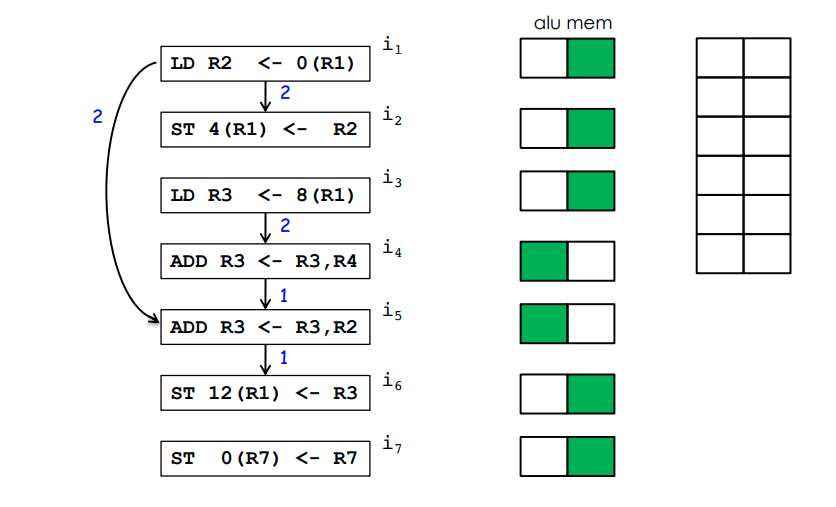
\includegraphics[width=0.8\textwidth]{p242.png}
	\caption{Basic Block Scheduling Example}
	\label{fig:p242}
\end{figure}




\subsection{Data-precedence graph}


A data dependency\cite{Datadepe9:online} in computer science is a situation in which a program statement (instruction) refers to the data of a preceding statement. In compiler theory, the technique used to discover data dependencies among statements (or instructions) is called dependence analysis.


\subsubsection{Flow dependency (True dependency)}

A Flow dependency, also known as a data dependency or true dependency or read-after-write (RAW), occurs when an instruction depends on the result of a previous instruction: also known as name dependency


\begin{center}
	1. A = 3\\
	2. B = A\\
	3. C = B
\end{center}
Instruction 3 is truly dependent on instruction 2, as the final value of C depends on the instruction updating B. Instruction 2 is truly dependent on instruction 1, as the final value of B depends on the instruction updating A. Since instruction 3 is truly dependent upon instruction 2 and instruction 2 is truly dependent on instruction 1, instruction 3 is also truly dependent on instruction 1. Instruction level parallelism is therefore not an option in this example.

\subsubsection{Anti-dependency}
An anti-dependency, also known as write-after-read (WAR), occurs when an instruction requires a value that is later updated. In the following example, instruction 2 anti-depends on instruction 3 — the ordering of these instructions cannot be changed, nor can they be executed in parallel (possibly changing the instruction ordering), as this would affect the final value of A.
\begin{center}
	1. B = 3 \\
	2. A = B + 1 \\
	3. B = 7
\end{center}

Example :
\begin{center}
	MUL R3,R1,R2 \\
	ADD R2,R5,R6
\end{center}
It is clear that there is anti-dependence between these 2 instructions. At first we read R2 then in second instruction we are Writing a new value for it.

An anti-dependency is an example of a name dependency. That is, renaming of variables could remove the dependency, as in the next example:
\begin{center}
	1. B = 3 \\
	N. B2 = B \\
	2. A = B2 + 1 \\
	3. B = 7
\end{center}
A new variable, B2, has been declared as a copy of B in a new instruction, instruction N. The anti-dependency between 2 and 3 has been removed, meaning that these instructions may now be executed in parallel. However, the modification has introduced a new dependency: instruction 2 is now truly dependent on instruction N, which is truly dependent upon instruction 1. As flow dependencies, these new dependencies are impossible to safely remove.

\subsubsection{Output dependency}

An output dependency, also known as write-after-write (WAW), occurs when the ordering of instructions will affect the final output value of a variable. In the example below, there is an output dependency between instructions 3 and 1 — changing the ordering of instructions in this example will change the final value of A, thus these instructions cannot be executed in parallel.

\begin{center}
	1. B = 3 \\
	2. A = B + 1 \\
	3. B = 7
\end{center}
As with anti-dependencies, output dependencies are name dependencies. That is, they may be removed through renaming of variables, as in the below modification of the above example:

\begin{center}
	1. B2 = 3 \\
	2. A = B2 + 1 \\
	3. B = 7
\end{center}


A commonly used naming convention for data dependencies is the following: Read-after-Write or RAW (flow dependency), Write-After-Read or WAR (anti-dependency), or Write-after-Write or WAW (output dependency).

\subsection{The List Scheduling Algorithm}

Here we describe our implementation of list scheduling. First, the dpg is built as described in the previous
section. Next, priorities are assigned to each node in the graph. There are several different heuristics that
can be used to assign priorities. A common and effective strategy is to use the latency weighted depth of the
node \cite{gibbons1986efficient,landskov1980local}. The depth of a node n is the length (number of nodes) of the longest path in the dpg from n to
some leaf (including n and the leaf.) The latency weighted depth is computed the same way, but the nodes
along the path are weighted using the latency of the operation the node represents. The following formula
summarizes the priority computation for a node n:

$$
	\operatorname{priority}(n)=\max \left(\forall_{l \in \text { leaves }(D P G)} \forall_{p \in \operatorname{paths}(n, \ldots, l)} \sum_{p_i=n}^l \text { latency }\left(p_i\right)\right)
$$

Dynamic programming can be used to compute the priorities efficiently, and we take into consideration
the anti-edges described above:

$$
	\operatorname{priority}(n)=\left\{\begin{array}{cc}
		\operatorname{latency}(n)                                                                & \text { if } n \text { is a leaf. } \\
		\max \left(\operatorname{latency}(n)+\max _{(m, n) \in E}(\text { priority }(m)),\right. &                                     \\
		\left.\max _{(m, n) \in E^{\prime}}(\text { priority }(m))\right)                        & \text { otherwise. }
	\end{array}\right.
$$
The final phase is the actual list scheduling algorithm that constructs the schedule for the block. Starting
at cycle 0, the list scheduler places operations into the schedule cycle by cycle. Any operation that is “ready”
at cycle X (i.e. all its operands have been computed), is a candidate to be scheduled at cycle X. The priorities
computed in the previous step are used to determine which ready operation to schedule, by selecting the
highest priority operation first. Any tie in the priority of two operations is broken arbitrarily. The algorithm
is detailed in Figure \ref{fig:p170}. Through the rest of the paper we refer to this algorithm as ls.


\begin{figure}[H]
	\centering
	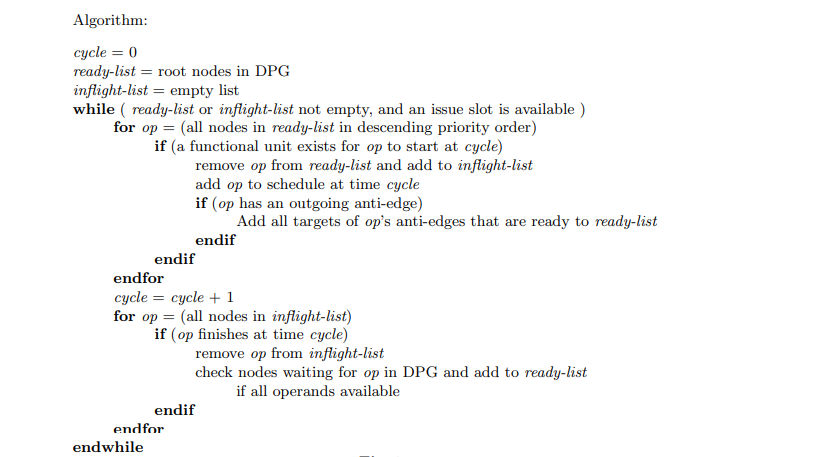
\includegraphics[width=0.8\textwidth]{p170.png}
	\caption{List Scheduling algorithm}
	\label{fig:p170}
\end{figure}


\subsection{List Scheduling Alternatives}

Here we present two alternatives to the ls algorithm discussed in the last section. For a survey of scheduling
techniques see . A machine learning approach to scheduling has been developed by Moss and others.



\subsubsection{Random Tie Breaking}

A traditional list scheduler returns a single solution by breaking any ties in the priority of two or more
operations arbitrarily. By running the list scheduler several times and breaking ties randomly, we could
potentially generate more and better solutions. Figure \ref{fig:p171} is an example from the tomcatv benchmark. Assume
all load immediates (LDI) take one cycle, all add operations (ADD) take two cycles, and the copy (i2i) takes
one cycle. Assume we are scheduling on a machine with two identical functional units. The numbers next
to the operations are the priority values that list scheduling uses. In this figure we see two different list
schedules that could be generated from the dpg. The second one requires one less cycle. The critical decision
comes in the second cycle, where the tie between the LDId and LDIc must be broken. Scheduling LDId early
enough results in a shorter schedule.

\begin{figure}[H]
	\centering
	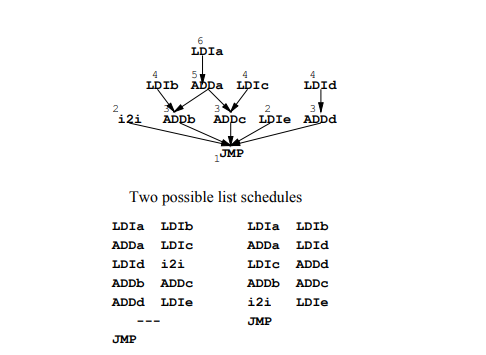
\includegraphics[width=0.6\textwidth]{p171.png}
	\caption{Example block from tomcatv}
	\label{fig:p171}
\end{figure}

\subsubsection{Backward list scheduling}
In addition, there are some blocks for which a backward list scheduler can generate a better solution. A
backward list scheduler works by reversing the direction of all edges in dpg, and scheduling the finish times
of each operation. (Note that the start time of operations must be used to ensure enough available functional
units for a given cycle.) This technique tends to cluster operations toward the end of the schedule instead
of the beginning like a forward list scheduler. For an example of a block that benefits from backward list
scheduling see Figure \ref{fig:p172}, which shows a block from the go benchmark. Assume there are two integer units
that can execute the LDI operations (one cycle), the LSL operation (one cycle), the ADD operations (two
cycles), ADDI operation (one cycle), and the CMP operation (one cycle). A separate memory unit executes
the ST operations (four cycles). All functional units are completely pipelined. A forward list scheduler will
schedule the four LDI operations and the the LSL before scheduling any of the ADD operations. This delays
the start of the higher latency store operations (ST). A better schedule can be found by a backward list
scheduler as shown in the example.

\begin{figure}[H]
	\centering
	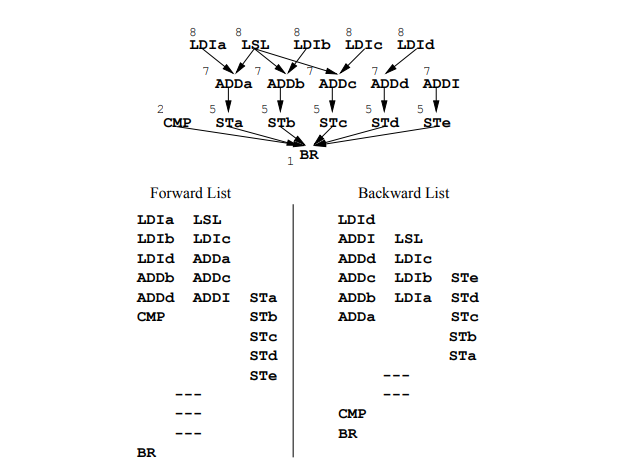
\includegraphics[width=0.6\textwidth]{p172.png}
	\caption{Example block from go, showing the benefits of backward list scheduling}
	\label{fig:p172}
\end{figure}


\subsection{Iterative Repair Scheduling}


Here we introduce the application of a repair based scheduling technique called “iterative repair” to the
problem of instruction scheduling in a compiler. This algorithm comes from the AI community and is described by Lin and
Kernighan\cite{lin1973effective}, and Zweben, et. al.\cite{zweben1992scheduling,zweben1992learning}. The technique has shown promise for several
scheduling problems including space shuttle mission scheduling.

The generalized algorithm is presented in Figure \ref{fig:p173}. The idea is straightforward. First, create an instruction
schedule that begins each operation as early as possible with respect to the precedence constraints of the dpg,
but ignores the resource constraints imposed by the limited number of processing elements. Now “repair” the
schedule by moving operations that have a resource conflict to a point later in the schedule. This reduces the
number of resource conflicts for the cycle being repaired. A resource conflict is simply a point in the schedule
where more operations are scheduled than the available number of functional units. The earliest cycle with a
conflict is found, and one of the conflicting operations is selected (line (1) in the algorithm). This operation
and all operations that depend on it are removed from the schedule (called unscheduling). The selected
operation and its dependent operations are then inserted back into the schedule (called rescheduling) at a
later point (line (2) in the algorithm). We continue repairing the schedule until there are no more resource
conflicts. The algorithm is run a “user specified” number of times, and the shortest schedule over all the
trials is selected as the final schedule.

We have tested several new variations of the iterative repair scheduling algorithm. The most effective
one to date we refer to as ir-bias. In ir-bias the selection of which node to move (called the move-node) is
not completely random. Rather, operations with lower priority values (the same priority values as used by
the list scheduler) are more likely to be moved. The selection is probabilistic; the probability that a node is
selected is inversely related to its priority.

The move-node is scheduled one cycle later than its original position. All successor nodes are rescheduled
as early-as-possible with respect to this new start time. This could cause additional conflicts to be created
later in the schedule, but a future repair will correct any new conflicts. After each repair we compare the
length of the new schedule to that of the old schedule. If the new length is greater, the repair is ignored,
the state of the previous schedule is restored, and a new move-node is selected. A new schedule with a
greater length than the previous schedule is kept ten per cent of the time to avoid local minima.
\begin{figure}[H]
	\centering
	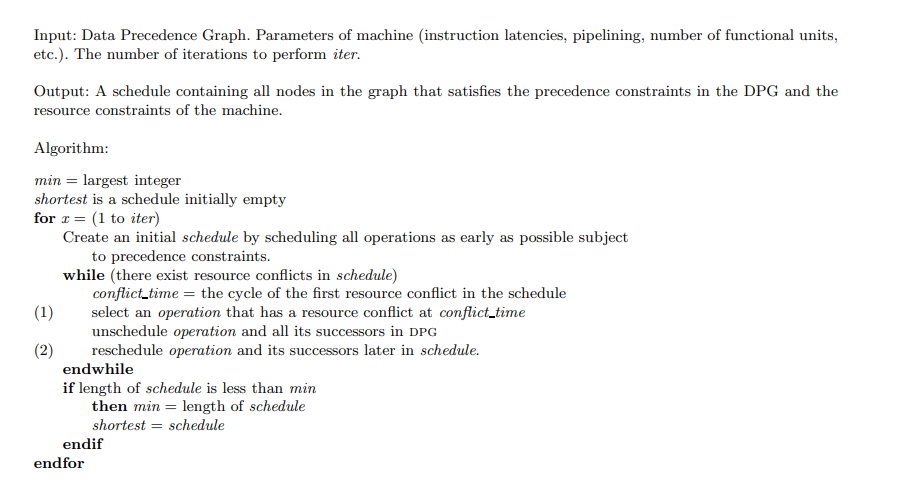
\includegraphics[width=\textwidth]{p173.png}
	\caption{Basic Iterative Repair Scheduling algorithm}
	\label{fig:p173}
\end{figure}
